% для компиляции в lualatex!!
%\documentclass[12pt, a4paper]{article}
\documentclass[12pt, a4paper]{disser}
\usepackage[english,russian]{babel}
\usepackage[warn]{mathtext}
%\usepackage[T2A]{fontenc}
%\usepackage[utf8]{inputenc}

\usepackage{xecyr} % Продукт Вашего покорного слуги ;)

%\setmainfont{DejaVu Serif}
\setmainfont{Liberation Serif}

\usepackage{color}
\usepackage{amssymb,amsmath}
\usepackage{graphicx}
\usepackage{multicol}

\textheight=24cm           % высота текста
\textwidth=16cm            % ширина текста
\oddsidemargin=0pt         % отступ от левого края
\topmargin=-1.5cm          % отступ от верхнего края
\parindent=24pt            % абзацный отступ
\parskip=0pt               % интервал между абзацами
\tolerance=2000            % терпимость к "жидким" строкам
\flushbottom               % выравнивание высоты страниц
%\def\baselinestretch{1.5} % печать с большим интервалом

%\title{}
%\author{\copyright~~С.А.~Назарова \thanks{e-mail:~sophia.nazarova@gmail.com}}
%\date{}


\begin{document}

	\section{Динамика обилия {\it M.~balthica}.}

		\subsection{Эстуарий реки~Лувеньги.}


На литорали в эстуарии р.~Лувеньги средняя плотность поселений маком за период с $1992$ по $2012$ год колебалась от $55~(26,8)$ в $1992$ до $9200~(39,8)$~экз./м$^2$ в $1998$ году (рис. \ref{ris:dynamic_Kandalaksha_all}). 
	\begin{figure}[h]
	
	\begin{minipage}[b]{.46\linewidth}
	%Фигурка в первом ряду слева размер отведенный под весь этот объект \textendash 0.46 от ширины строки
	%Параметр [b] означает, что выравнивание этих министраниц будет по нижнему краю
	\begin{center}
	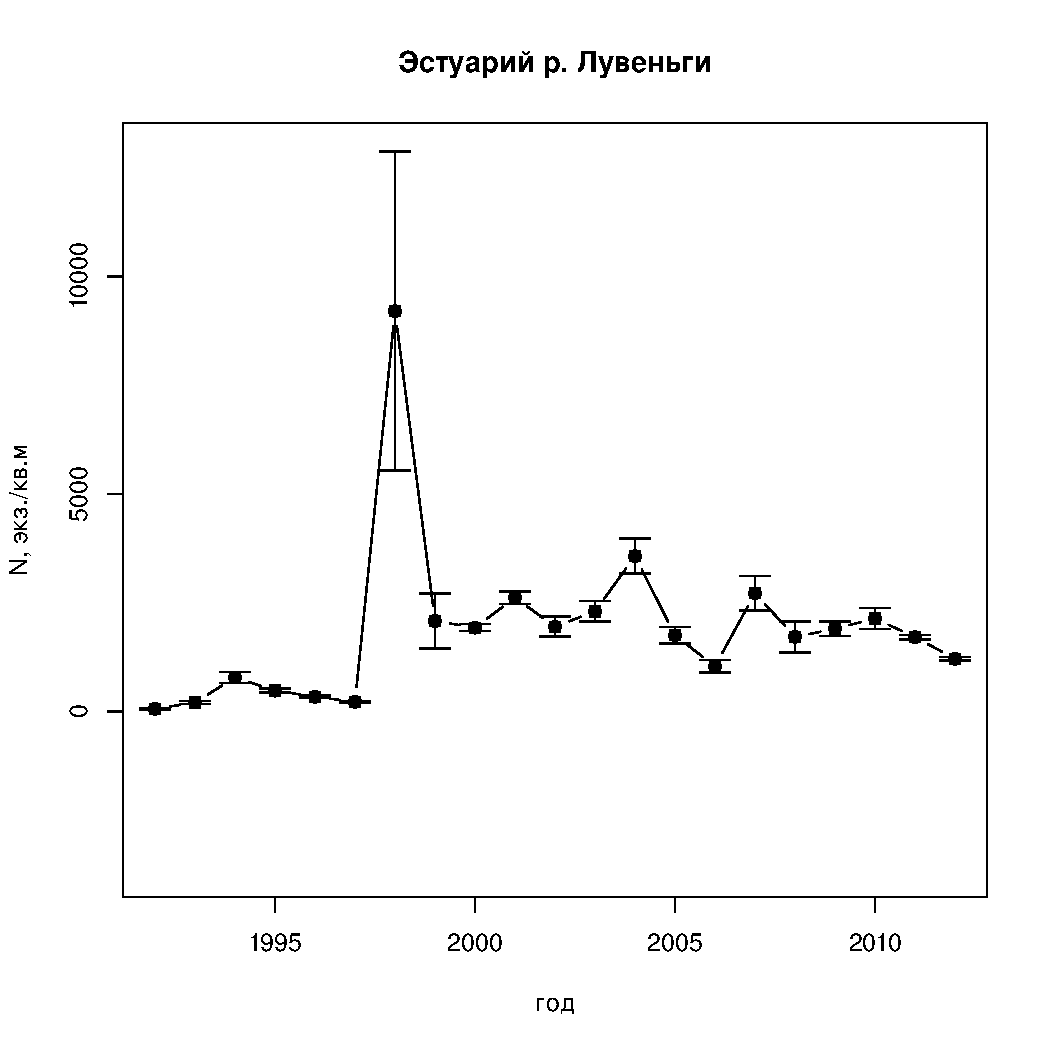
\includegraphics[width=65mm]{../White_Sea/Estuatiy_Luvenga/N_dynamic.pdf}

	\end{center}
	\end{minipage}
	%
	\hfil %Это пружинка отодвигающая рисунки друг от друга
	%
	\begin{minipage}[b]{.46\linewidth}
%Следующий рисунок - первый ряд справа %DUNGEON S_4 \ AB
	\begin{center}
		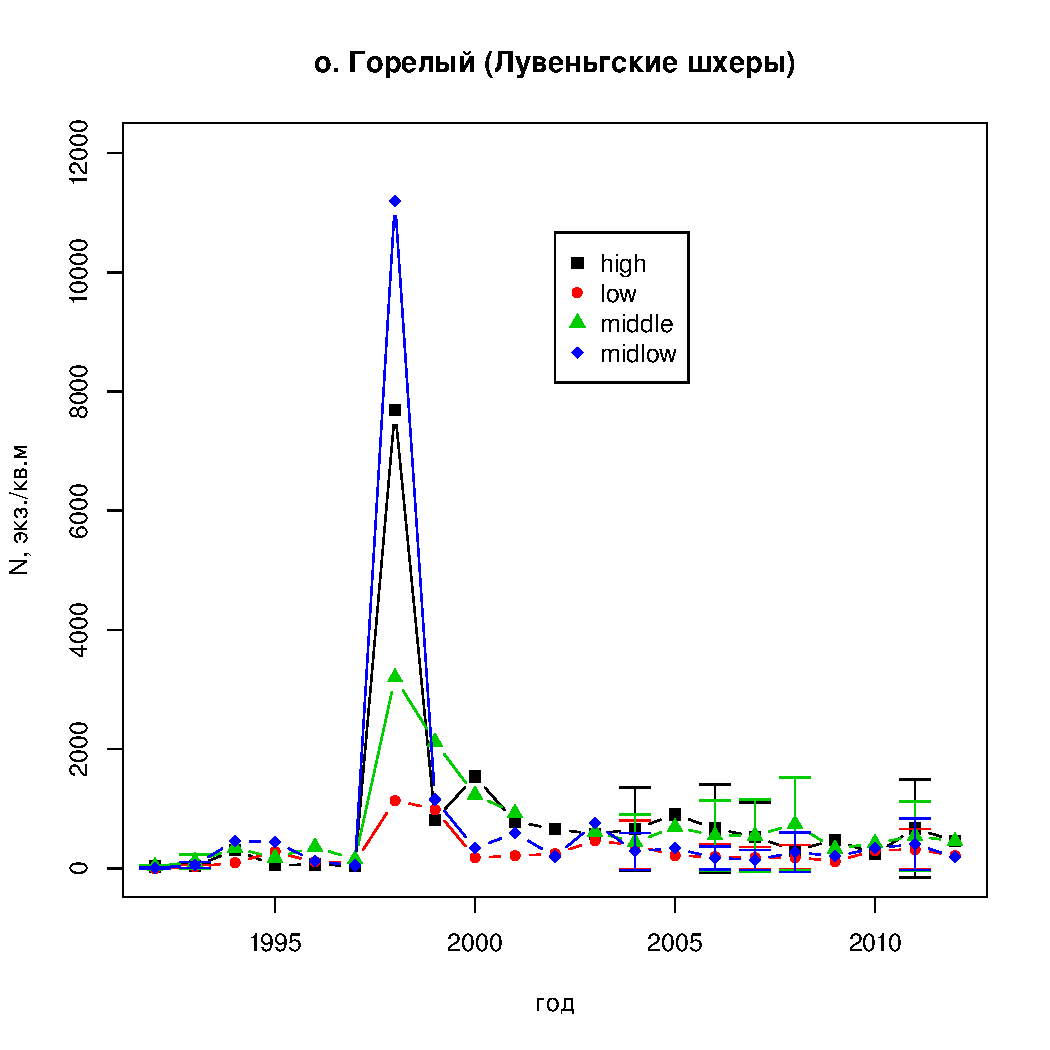
\includegraphics[width=65mm]{../White_Sea/Luvenga_Goreliy/N_dynamic.pdf}
	\end{center}
	\end{minipage}

%\smallskip


	\begin{minipage}[b]{.46\linewidth}
%Фигурка в первом ряду слева размер отведенный под весь этот объект \textendash 0.46 от ширины строки
%Параметр [b] означает, что выравнивание этих министраниц будет по нижнему краю
	\begin{center}
		\includegraphics[width=65mm]{../White_Sea//Luvenga_II_razrez/N_dynamic.pdf}
	\end{center}
	\end{minipage}
%
	\hfil %Это пружинка отодвигающая рисунки друг от друга
%
	\begin{minipage}[b]{.46\linewidth}
%Следующий рисунок - первый ряд справа %DUNGEON S_4 \ AB
	\begin{center}
		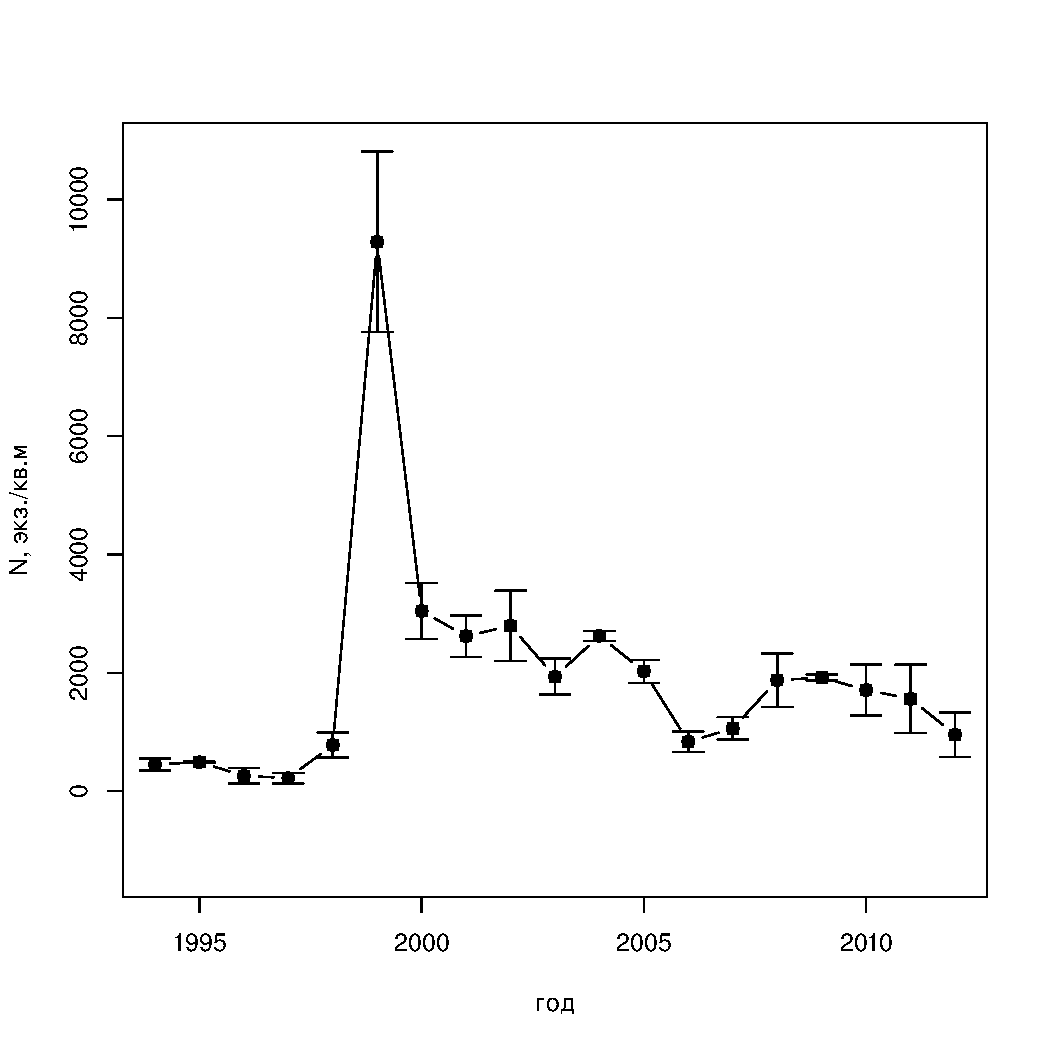
\includegraphics[width=65mm]{../White_Sea/Ryashkov_ZRS/N_dynamic.pdf}
	\end{center}
	\end{minipage}

%\smallskip

	\begin{minipage}[b]{.46\linewidth}
%Фигурка в первом ряду слева размер отведенный под весь этот объект \textendash 0.46 от ширины строки
%Параметр [b] означает, что выравнивание этих министраниц будет по нижнему краю
	\begin{center}
		\includegraphics[width=65mm]{../White_Sea/Ryashkov_YuG/N_dynamic.pdf}
	\end{center}
	\end{minipage}
%
	\hfil %Это пружинка отодвигающая рисунки друг от друга
%
	\begin{minipage}[b]{.46\linewidth}
%Следующий рисунок - первый ряд справа %DUNGEON S_4 \ AB
	\begin{center}
		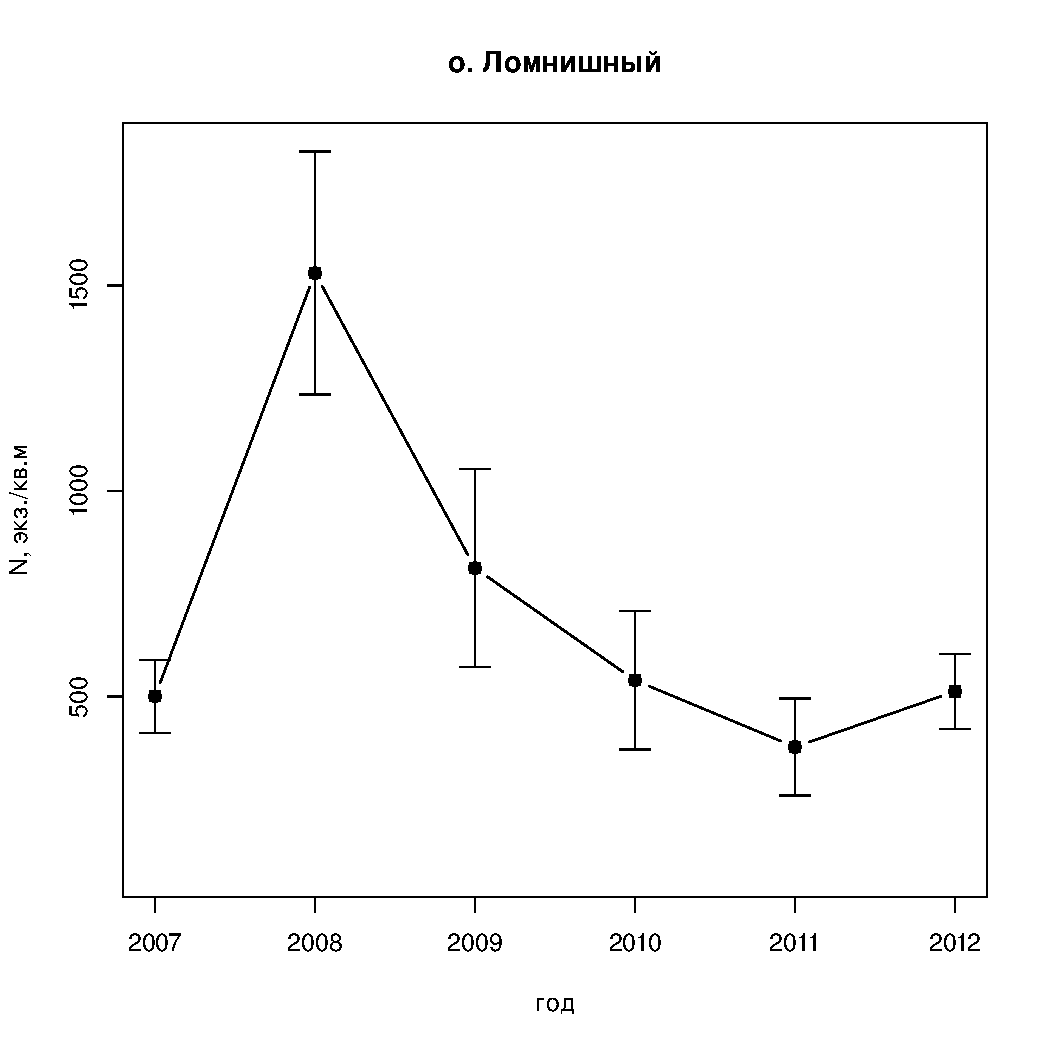
\includegraphics[width=65mm]{../White_Sea/Lomnishniy/N_dynamic.pdf}
	\end{center}
	\end{minipage}

%\smallskip


	\caption{Динамика плотности поселений {\it Macoma balthica} в вершине Кандалакшского залива}
	\label{ris:dynamic_Kandalaksha_all}
	\end{figure}
При этом столь высокая численность в $1998$ году была связана с особями длиной менее $1$~мм (рис. \ref{ris:dynamic_Kandalaksha_all2}) \textemdash средняя численность моллюсков крупнее $1$~мм составляла всего $750~(2,03)$~экз./м$^2$.
	\begin{figure}[h]

	\begin{minipage}[b]{.46\linewidth}
%Фигурка в первом ряду слева размер отведенный под весь этот объект \textendash 0.46 от ширины строки
%Параметр [b] означает, что выравнивание этих министраниц будет по нижнему краю
	\begin{center}
		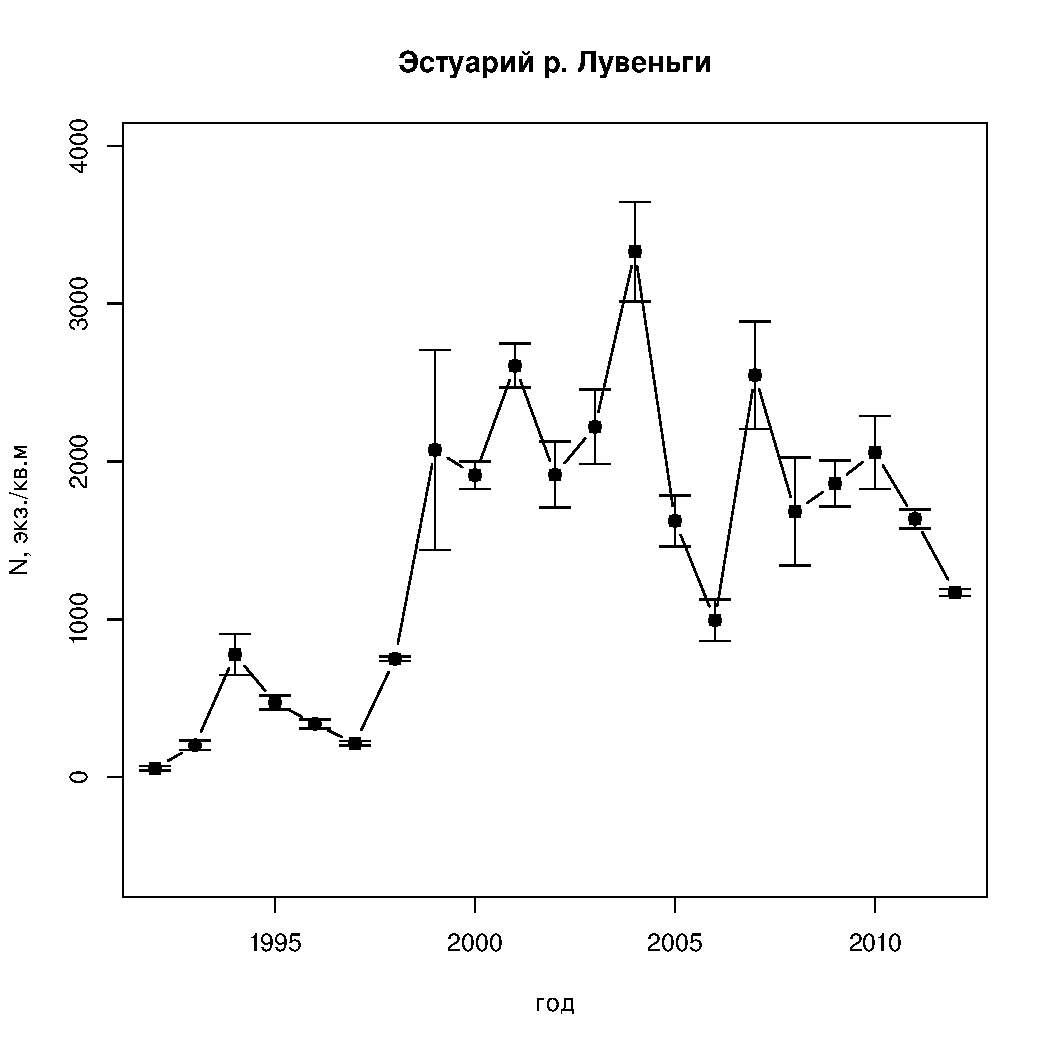
\includegraphics[width=65mm]{../White_Sea/Estuatiy_Luvenga/N2_dynamic.pdf}
	\end{center}
	\end{minipage}
%
	\hfil %Это пружинка отодвигающая рисунки друг от друга
%
	\begin{minipage}[b]{.46\linewidth}
%Следующий рисунок - первый ряд справа %DUNGEON S_4 \ AB
	\begin{center}
		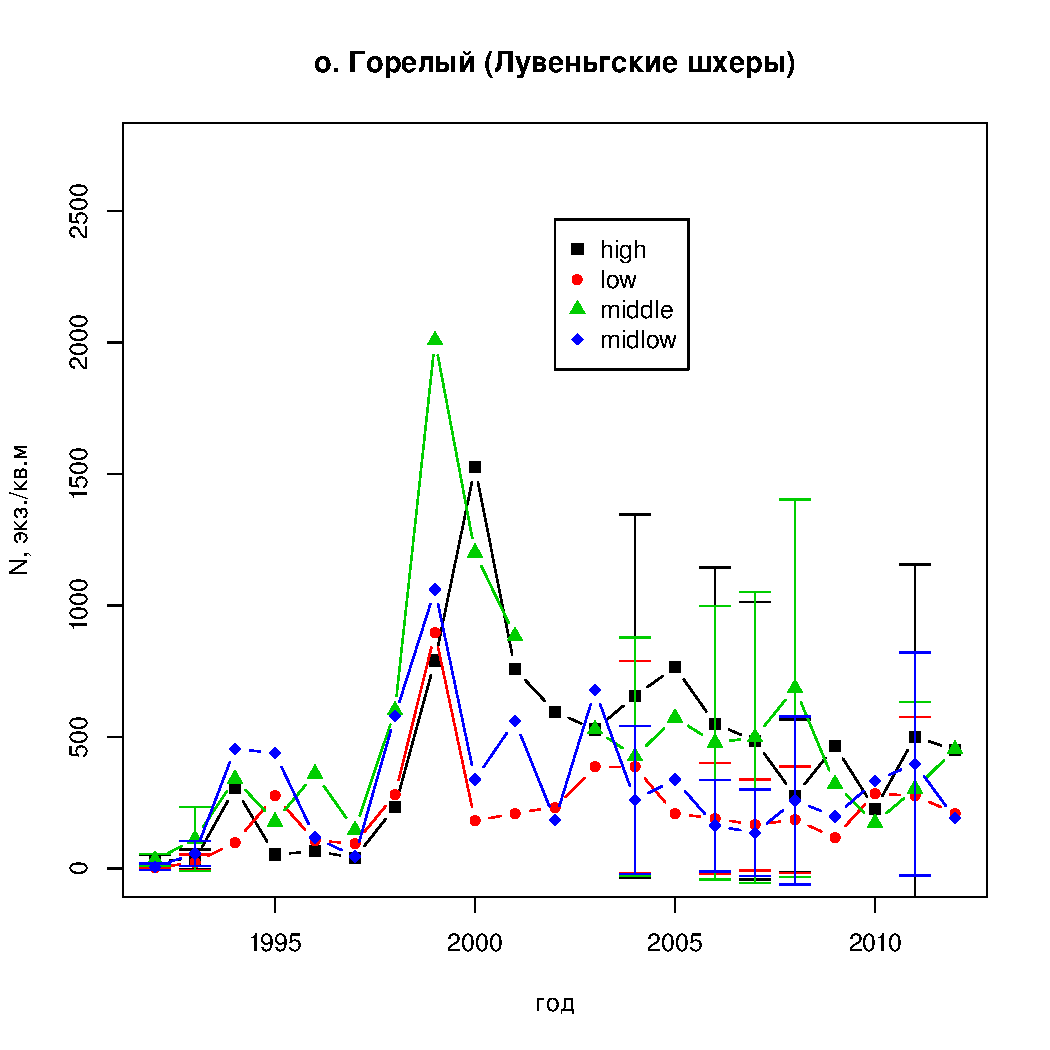
\includegraphics[width=65mm]{../White_Sea/Luvenga_Goreliy/N2_dynamic.pdf}
	\end{center}
	\end{minipage}
%\smallskip
	\begin{minipage}[b]{.46\linewidth}
%Фигурка в первом ряду слева размер отведенный под весь этот объект \textendash 0.46 от ширины строки
%Параметр [b] означает, что выравнивание этих министраниц будет по нижнему краю
	\begin{center}
		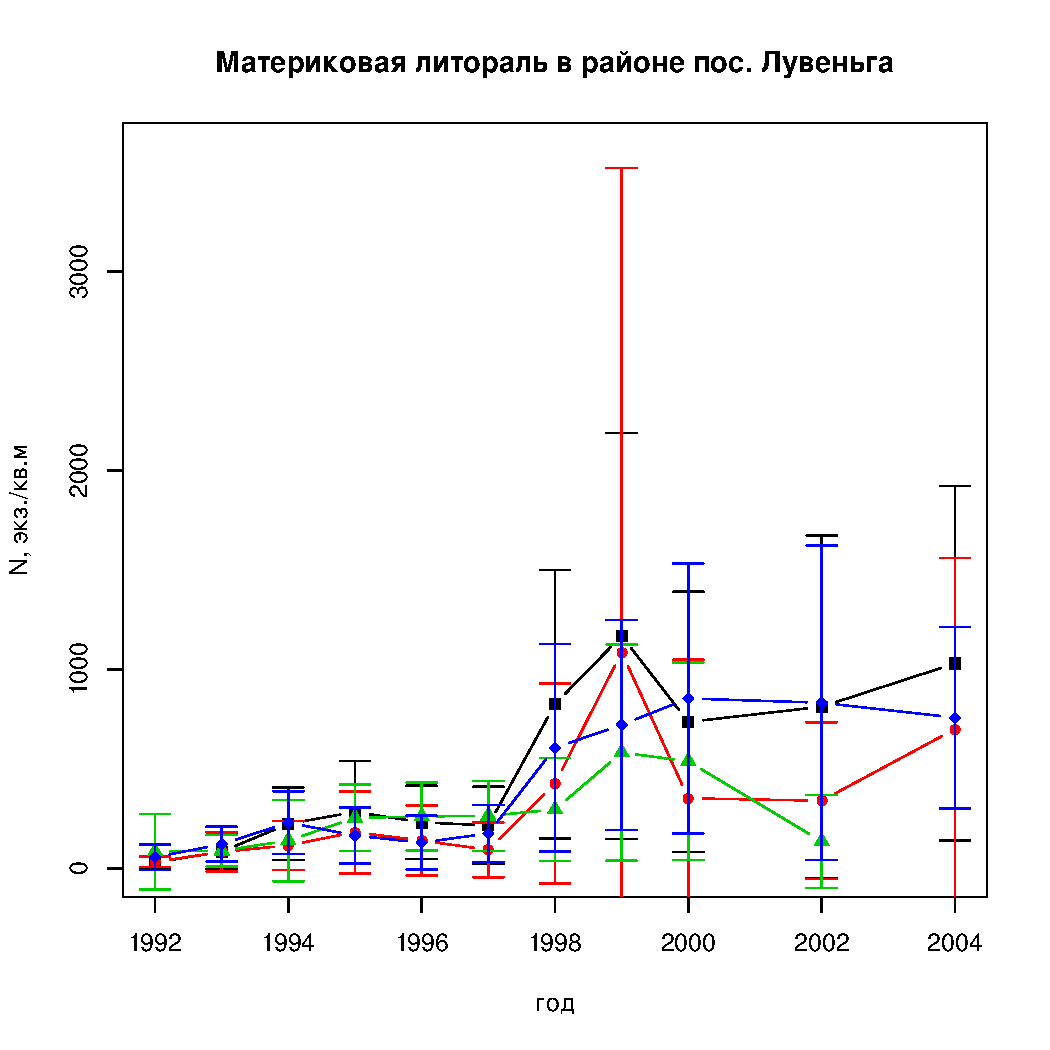
\includegraphics[width=65mm]{../White_Sea//Luvenga_II_razrez/N2_dynamic.pdf}
	\end{center}
	\end{minipage}
%
	\hfil %Это пружинка отодвигающая рисунки друг от друга
%
	\begin{minipage}[b]{.46\linewidth}
%Следующий рисунок - первый ряд справа %DUNGEON S_4 \ AB
	\begin{center}
		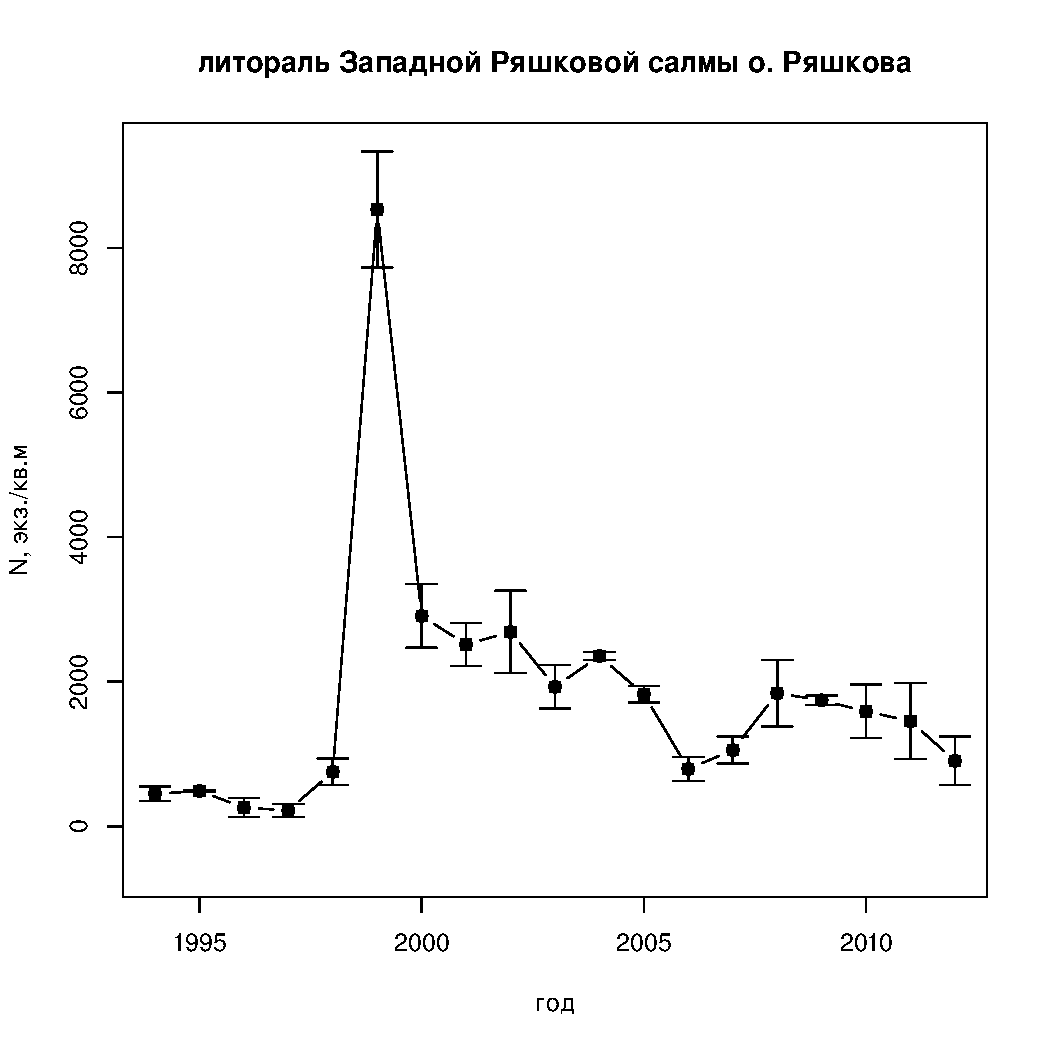
\includegraphics[width=65mm]{../White_Sea/Ryashkov_ZRS/N2_dynamic.pdf}
	\end{center}
	\end{minipage}
%\smallskip
	\begin{minipage}[b]{.46\linewidth}
%Фигурка в первом ряду слева размер отведенный под весь этот объект \textendash 0.46 от ширины строки
%Параметр [b] означает, что выравнивание этих министраниц будет по нижнему краю
	\begin{center}
		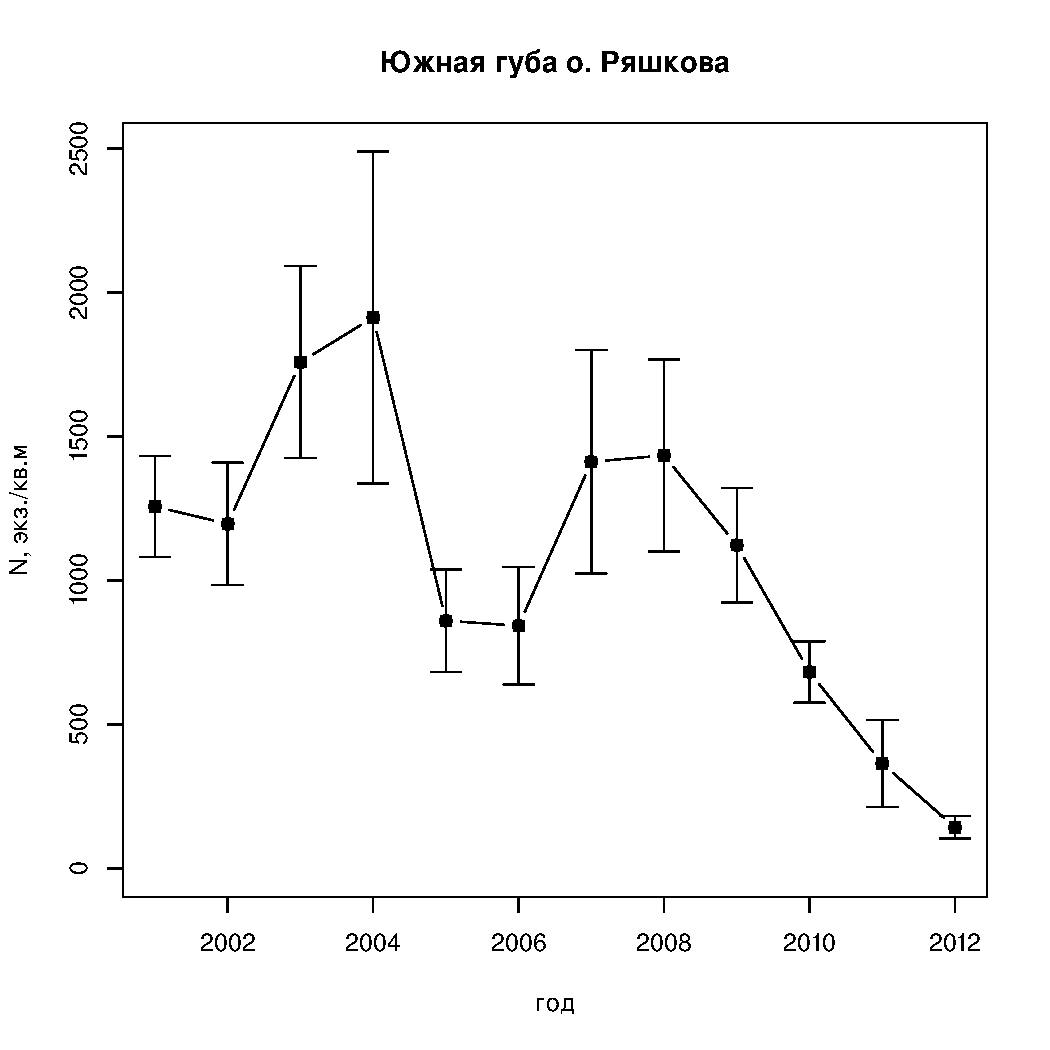
\includegraphics[width=65mm]{../White_Sea/Ryashkov_YuG/N2_dynamic.pdf}
	\end{center}
	\end{minipage}
%
	\hfil %Это пружинка отодвигающая рисунки друг от друга
%
	\begin{minipage}[b]{.46\linewidth}
%Следующий рисунок - первый ряд справа %DUNGEON S_4 \ AB
	\begin{center}
		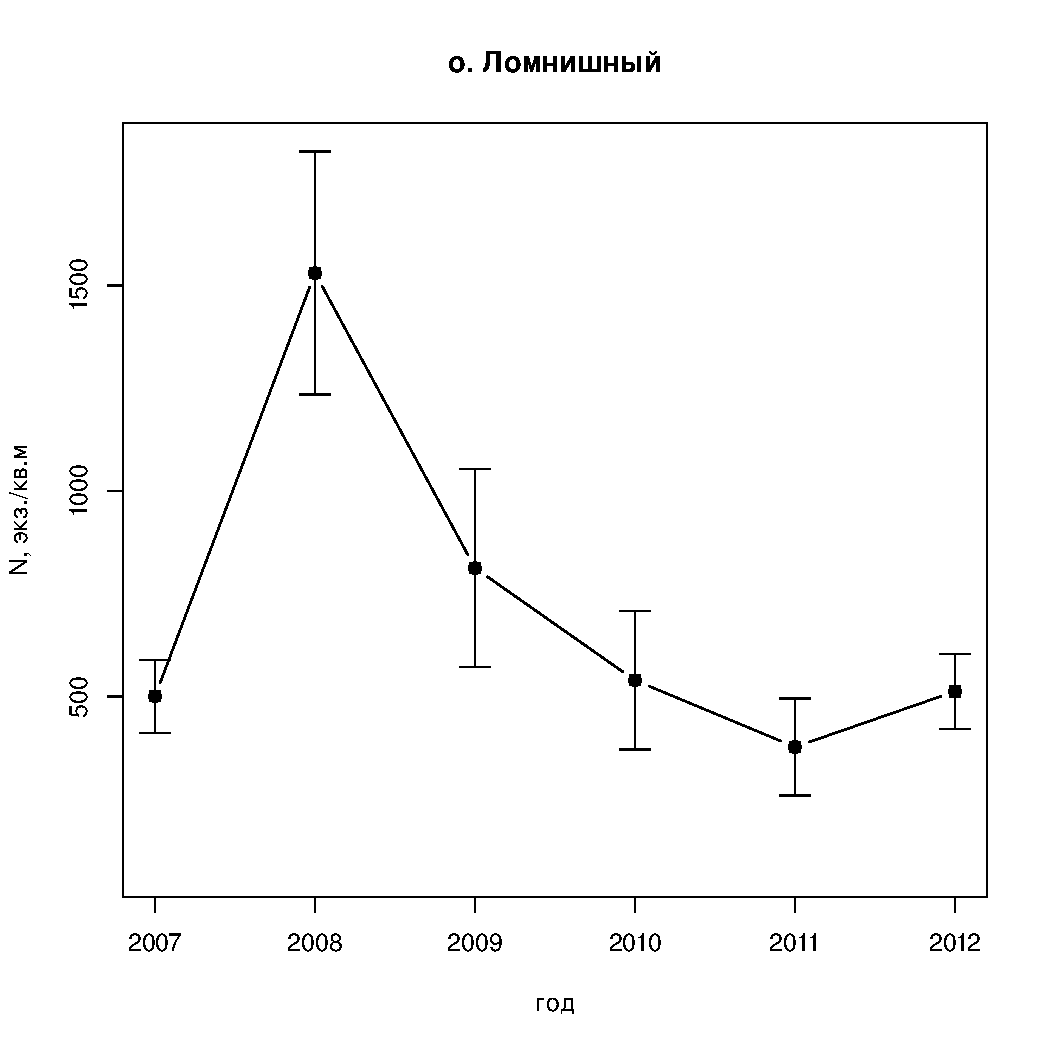
\includegraphics[width=65mm]{../White_Sea/Lomnishniy/N2_dynamic.pdf}
	\end{center}
	\end{minipage}

%\smallskip


	\caption{Динамика численности {\it Macoma balthica} с длиной раковины более $1$~мм в поселениях вершины Кандалакшского залива}
	\label{ris:dynamic_Kandalaksha_all2}
	\end{figure}



Для анализа динамики обилия, на наш взгляд, более информативно рассматривать численность без учета вновь осевших особей. 
\textcolor{red}{ОБЪЯСНЯТЬ ПРО ПОПОЛНЕНИЕ ПОСЕЛЕНИЯ ТУТ ИЛИ ГДЕ?}. 
Поскольку материал собирали в конце июля \textemdash начале августа, то мы считаем спатом всех особей длиной менее $1$~мм. \textcolor{red}{сюда бы ссылку на размер спата в белом? Зубаха, Полоскин, Гольцев? Флячинская?} 
В этом случае можно говорить по крайней мере о двух периодах: с $1992$ по $1998$ год \textemdash период относительно низкой численности (менее $800$~экз./м$^2$ ) моллюсков, и с $1999$ по $2012$ год \textemdash относительно высокой (более $1000$~экз./м$^2$) (достоверные различия по критерию Манна-Уитни, $W = 6, p-value = 4,5 \times 10^{-13}$) (рис.~\ref{ris:dynamic_Kandalaksha_all2}).

В период с $1992$ по $1998$ год численность {\it M.~balthica} достоверно изменялась ($Kruskal-Wallis\ \chi^2 = 24,1, p-value = 0,00049$). Результаты попарного сравнения представлены в таблице \ref{tab:Tukey_estuary_92_98_n2}.

	\begin{table}
	\begin{tabular}{|*{4}{p{0.2\textwidth}|}} \hline
	годы & различия средних & p-value & достоверность различий\\
	\hline
	$1993-1992$ & $147$ &  $0,11$ & \\
	\hline
	$1994-1993$ & $575$  & $2,47 \times 10^{-7}$ & *** \\
	\hline
	$1995-1994$ & $-303$  & $0,0069$ & ** \\
	\hline
	$1996-1995$ & $-137$  & $0,51$ & \\
	\hline
	$1997-1996$ & $-123$  & $0,62$ & \\
	\hline
	$1998-1997$ & $537$  & $6,73 \times 10^{-6}$ & *** \\
	\hline
	\end{tabular}

	{\footnotesize Примечание: достоверность различий *** \textemdash $p<0,001$; ** \textemdash $p<0,05$; * \textemdash $p<0,1$.}
	\caption{Результаты множественного сравнения средних численностей {\it Macoma balthica} методом Тьюки (Tukey's ‘Honest Significant Difference’) в эстуарии реки Лувеньги в $1992-1998$ годах.}
	\label{tab:Tukey_estuary_92_98_n2}
	\end{table}

Численность моллюсков в эстуарии р. Лувеньги в $1992-1993$ годах оставалась стабильной ($\bar{N} = 128~(21,5)$~экз./м$^2$), затем произошло ее увеличение в $1994$ году, после чего снова произошло некоторое ее снижение и в $1995 - 1997$ годах она стабилизировалась на более высоком уровне ($\bar{N} = 341~(9,3)$~экз./м$^2$) по сравнению с $1992 - 93$ гг.
В $1998$ году вновь происходит увеличение численности {\it M.~balthica} до уровня $1994$ года (около $750 - 800$~экз./м$^2$), после чего в $1999$ году средняя численность возросла ещё в три раза.
С $1999$ по $2003$ год численность оставалась относительно стабильной  ($Kruskal-Wallis\ \chi^2 = 5,0, p-value = 0,28$) и в среднем составляла $2146~(5,5)$~экз./м$^2$.
В $2004$ году обилие маком увеличилось в полтора раза и достигло максимума для данного участка за весь период наблюдений. 
С $2004$ по $2006$ год численность моллюсков последовательно снижалась (табл.~\ref {tab:Tukey_estuary_04_07_n2}). 
	\begin{table}
	\begin{tabular}{|*{4}{p{0.2\textwidth}|}} \hline
	годы & различия средних & p-value & достоверность различий\\
	\hline
	$2005-2004$ & $-1707$ & $0,09$ & *\\
	\hline
	$2006-2005$ & $-630$ & $0,78$ & \\
	\hline
	$2007-2006$ & $1553$ & $0,05$ & **\\
	\hline
	\end{tabular}

	{\footnotesize Примечание: достоверность различий *** \textemdash $p<0,001$; ** \textemdash $p<0,05$; * \textemdash $p<0,1$.}
	\caption{Результаты множественного сравнения средних численностей {\it Macoma balthica} методом Тьюки (Tukey's ‘Honest Significant Difference’) в эстуарии реки Лувеньги в $2004-2007$ годах.}
	\label{tab:Tukey_estuary_04_07_n2}
	\end{table}
В $2006$ году она достигла локального минимума и составляла $993~(13,2)$~экз./м$^2$). 
В $2007$ году произошло достоверное увеличение численности {\it Macoma balthica} (табл.~\ref {tab:Tukey_estuary_04_07_n2}).
К $2008$ году численность моллюсков снова снижается, после чего до $2012$ года были отмечены недостоверные флуктуации ($Kruskal-Wallis\ \chi^2 = 6,8429, p-value = 0,14$).

		\subsection{Илистая губа острова Горелый.}
\textcolor{red}{посчитать и вписать относительные ошибки}
На данном участке рассматривали отдельно 4 зоны, различающиеся по осушке и биотическим условиям. 
Максимальная численность маком на всех горизонтах литорали была отмечена в $1998$ году (рис.~\ref{ris:dynamic_Kandalaksha_all}).
Более чем на 75\% такая высокая численность была связана с обилием особей длиной менее $1$~мм.
Максимальная численность моллюсков наблюдалась на границе среднего и нижнего горизонта в зарослях фукоидов, здесь она составляла более $11$~тысяч~экз./м$^2$.

При исключении из анализа особей размером менее $1$~мм, численность особей {\it M.~balthica} стала максимальной в $1999$ году для всех горизонтов, кроме среднего, на котором максимальная численность отмечена в $2000$ году (рис.~\ref{ris:dynamic_Kandalaksha_all2}).
Самая низкая чиленность за весь период исследований была отмечена в начале интервала наблюдений ($1992-1993$~года) \textemdash менее $100$~экз./м$^2$.
С $1994$ по $1996$~год происходило некоторое увеличение численности маком, однако она на всех горизонтах не превышала $500$~экз./м$^2$.
В $1997$ году произошло локальное снижение численности, и c $1998$~года происходил ее рост. 
В $1999$ году численность маком составляла $900$, $2000$ и $1050$~экз./м$^2$ на среднем горизонте, в поясе фукоидов и у нуля глубин, соответсвенно.
В $2000$ году на верхнем горизонте литорали численность особей достиглаа максимума за весь период наблюдений и составила  $1500$~экз./м$^2$, в то время как на остальных горизонтах литорали произошло снижение численности.
В дальнейшем были отмечены менее значительные колебания, и, как показывают данные в $2004$, $2006 - 2008$ и $2011$ годах (когда на станциях брали индивидуальные пробы, а не интегрированные) эти колебания недостоверны (табл.~\ref{tab:Goreliy_N2_Kruskal}).

	\begin{table}
	\begin{tabular}{|*{4}{p{0.25\textwidth}|}} \hline
	горизонт литорали & $Kruskal-Wallis\ \chi^2$ & $p-value$ & $\bar{N} ~ (D)$ \\ 
	\hline
	верхний & $0,91$ & $0,92$ & $1972~(11,4)$ \\
	\hline
	средний & $1,37$ & $0,85$ & $1910~(9,0)$\\
	\hline
	пояс фукоидов & $2,13$ & $0,71$ & $970~(13,7)$ \\
	\hline
	нижний & $3,45$ & $0,49$ & $960~(10,6)$ \\
	\hline
	\end{tabular}
	{\footnotesize Примечание: Kruskal-Wallis $\chi^2$ \textemdash значения критерия Краскелл-Уоллиса; $\bar{N}$ \textemdash средняя численность {\it 	M.~balthica}, экз./м$^2$; $D$ \textemdash относительная ошибка средней, \%.}
	\caption{Межгодовое различие численности {\it Macoma~balthica} на литорали о.~Горелый по данным $2004$, $2006 - 2008$ и $2011$ годов.}
	\label{tab:Goreliy_N2_Kruskal}
	\end{table}


		\subsection{Материковая литораль в районе пос. Лувеньга}

На материковой литорали в районе поселка Лувеньга отдельно рассматривали динамику поселений {\it M.~balthica} в четырех зонах, отличающихся по осушке и биотическим условиям.
За весь период наблюдений максимальные флуктуации численности маком были отмечены для зоны верхнего пляжа: от $94~(38~\%)$~экз./м$^2$ в $1992$ до $16365~(53~\%)$~экз./м$^2$ в $1998$ году (\ref{ris:dynamic_Kandalaksha_all}). 
Доля спата в большинстве выборок составляет менее $20~\%$, исключение составляет зона верхнего пляжа в $1998$, где доля спата была $87~\%$.
В дальнейшем мы рассматриваем динамику обилия без учета спата (рис.~\ref{ris:dynamic_Kandalaksha_all2}).

В начале периода наблюдения численность на всех трех участках не превышала $1000$~экз./м$^2$ и колебания носили случайный характер (табл.~\ref{tab:2razrez_N2_Kruskal}).

	\begin{table}
	\begin{tabular}{|*{4}{p{0.25\textwidth}|}} \hline
	зона & $Kruskal-Wallis\ \chi^2$ & $p-value$ & $\bar{N} ~ (D)$ \\ 
	\hline
	верхний пляж & $3,57$ & $0,61$ & $477~(16,6)$ \\
	\hline
	пояс фукоидов & $12,8$ & $0,02$ & $ $\\
	\hline
	пояс зостеры & $2,13$ & $0,71$ & $970~(13,7)$ \\
	\hline
	нижний пляж & $3,45$ & $0,49$ & $960~(10,6)$ \\
	\hline
	\end{tabular}
	{\footnotesize Примечание: Kruskal-Wallis $\chi^2$ \textemdash значения критерия Краскелл-Уоллиса; $\bar{N}$ \textemdash средняя численность {\it 	M.~balthica}, экз./м$^2$; $D$ \textemdash относительная ошибка средней, \%.}
	\caption{Межгодовое различие численности {\it Macoma~balthica} на материковой литорали в районе поселка Лувеньга с $1992$ по $1998$ год.}
	\label{tab:2razrez_N2_Kruskal}
	\end{table}


		\subsection{Литораль Западной Ряшковой салмы о.~Ряшкова.}

На данном участке литорали средняя плотность поселений {\it M.~balthica} за период с $1994$ по $2012$ год колебалась от $220~(40,9)$~экз./м$^2$ в $1997$ до $9285~(16,4)$~экз./м$^2$ в $1999$~году (рис. \ref{ris:dynamic_Kandalaksha_all}).
При исключение из рассмотрения особей длиной менее $1$~мм минимальная средняя численность не изменилась, а максимальная в $1999$ составила $8530~(9,4)$~экз./м$^2$ (рис. \ref{ris:dynamic_Kandalaksha_all2}).
Однако столь высокая численность не сохранилась дольше одного года, и в период с $2000$ по $2012$ колебалась в пределах $1 \textendash 2,5$~тысяч~экз./м$^2$, в среднем составляя $1823~(8,0)$~экз./м$^2$.
Тем не менее, после $1999$ года средняя численность маком достоверно больше ($W = 4,5, p-value = 1,007 \times 10^{-5}$), чем до \textemdash $2145~(4,5)$ и $435~(17,2)$, соответственно.

Минимальная численность в период после $2000$~года была отмечена в 2006 году и составляла $795~(20,8)$~экз./м$^2$. 
Периоды с $2000$ по $2006$ и с $2007$ по $2012$ годы достоверно различаются ($W = 131,5, p-value = 0,016$) по средней численности маком ($2146~(9,5)$ и $1448~(10,8)$, соответственно).

Внутри каждого периода времени численность {\it M.~balthica} не различается достоверно от года к году (табл. \ref{tab:ZRS_N2_Kruskal}).

	\begin{table}
	\begin{tabular}{|*{4}{p{0.25\textwidth}|}} \hline
	годы наблюдения & $Kruskal-Wallis\ \chi^2$ & $p-value$ & $\bar{N} ~ (D)$ \\ 
	\hline
	$1994 - 1998$ & $7,2$ & $0,12$ & $435~(17,2)$ \\
	\hline
	$2000 - 2006$ & $9,8$ & $0,13$ & $2146~(9,5)$\\
	\hline
	$2007 - 2012$ & $4,9$ & $0,43$ & $1448~(10,8)$ \\
	\hline
	\end{tabular}
	{\footnotesize Примечание: Kruskal-Wallis $\chi^2$ \textemdash значения критерия Краскелл-Уоллиса; $\bar{N}$ \textemdash средняя численность {\it 	M.~balthica}, экз./м$^2$; $D$ \textemdash относительная ошибка средней, \%.}
	\caption{Межгодовое различие численности {\it Macoma~balthica} на литорали Западной Ряшковой салмы о.~Ряшкова в разные годы.}
	\label{tab:ZRS_N2_Kruskal}
	\end{table}


		\subsection{Южная губа острова Ряшкова}
Поскольку на литорали Южной губы о.~Ряшкова использовали для промывки сито с диаметром ячеи $1$~мм, то доля моллюсков размером менее $1$~мм не превышала $1,2~\%$ и их исключение из анализа не изменило общей картины.
На данном участке с $2001$ по $2010$ год численность {\it Macoma~balthica} была относительно стабильна, все флуктуации были недостоверны ($Kruskal-Wallis\ \chi^2 = 12,07, p-value = 0,21$). 
Средняя численность за данный период составила $1239~(7,9)$~экз./м$^2$.
Однако намечается некоторая тенденция к увеличению численности в $2003-2004$ и $2007-2008$ году.
После $2008$ года численность постепенно снижается и в $2012$ году она составила $142~(27,5)$~экз./м$^2$.

		\subsection{Остров Ломнишный}
На литорали о.~Ломнишный для промывки также использовали сито с диаметром ячеи $1$~мм, моллюски длиной менее 1 мм в пробах отсутствовали.
На данном участке численность маком оставалась относительно стабильной в течении всего периода исследований ($Kruskal-Wallis\ \chi^2 = 9,9, p-value = 0,077$) и в среднем составляла $638~(12)$~экз./м$^2$.
Некоторое увеличение численности было отмечено в $2008$ году (численность составляла $1530~(19)$~экз./м$^2$).


		\subsection{Дальний пляж губы Дальнезеленецкая}
На данном участке использовали для промывки сито с диаметром ячеи $1$~мм и особи длиной менее $1$~мм в пробах отмечены не были. 
В течении всего периода времени плотность поселения {\it Macoma balthica} не превышала $100$~экз./м$^2$ (\ref{ris:dynamic_Zelency}). 
	\begin{figure}[h]
		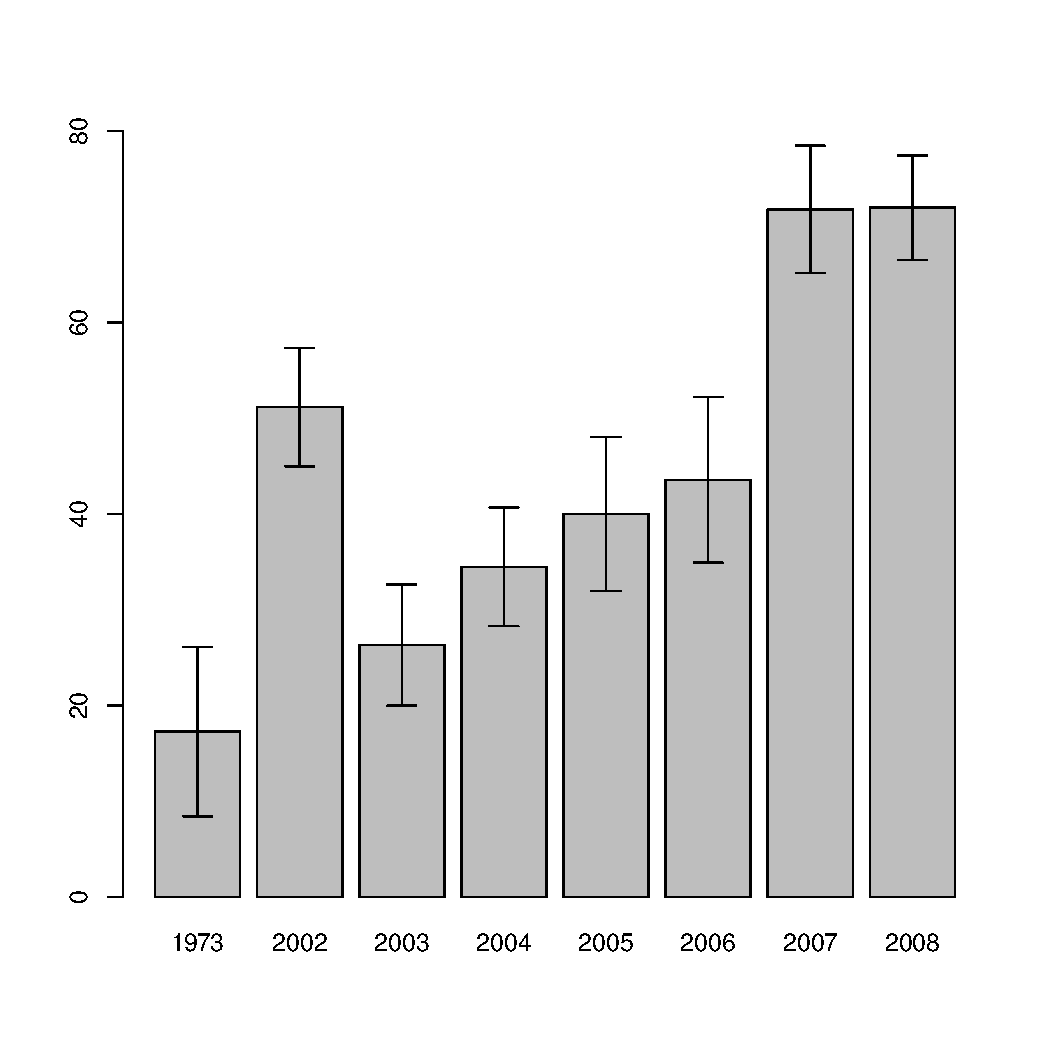
\includegraphics{../Barenc_Sea/Dalnezeleneckaya/N_dynamic_with_Agarova.pdf}
	\caption{Динамика плотности поселений {\it Macoma balthica} на литорали Дальнего пляжа г.~Дальнезеленецкой (Баренцево море)}
{\footnotesize Примечание: по оси $X$ \textemdash годы наблюдений, по оси $Y$ \textemdash средняя плотность поселения,~экз./м$^2$. Данные $1973$ года взяты из статьи \ref{Agarova_et_al_1976}}
	\label{ris:dynamic_Zelency}
	\end{figure}
В $2003$ году произошло уменьшение обилия маком (с $52~(13)$ до $34~(20)$~экз./м$^2$, критерий Манна-Уитни  $W = 854, p-value = 0,001$), после чего численность  в $2003 - 2006$ оставалась относительно стабильной (в среднем $33~(0,8)$~экз./м$^2$, критерий Краскела-Уоллиса $Kruskal-Wallis \chi^2 = 4,03, p = 0,26$). 
В $2007$ году численность еще увеличилась относительно предыдущего периода ($W = 1155, p-value = 8,7 \times 10^{-8}$) и оставалась стабильной к $2008$ году ($W = 516,5, p-value = 0,76$) при этом достигла уровня, максимального для всего периода ($72~(0,9)$~экз./м$^2$).

В качестве точки сравнения использовали количественные данные из статьи \ref{Agarova_et_al_1976} (\ref{ris:dynamic_Zelency}). 
Плотность поселения {\it Macoma balthica} на Дальнем пляже в $1973$ году была сравнима с таковой в $2002-2006$ годах (\ref{tab:DZ_N_1973_sravnenie}).
	\begin{table}
	\begin{tabular}{|*{4}{p{0.25\textwidth}|}} \hline
	годы сравнения & $W$ & $p-value$ & достоверность различий \\ 
	\hline
	$1973 - 2002$ & $31,5$ & $0,08$ & *\\
	\hline
	$1973 - 2003$ & $80,5$ & $0,86$ & \\
	\hline
	$1973 - 2004:2006$ &  $214$ & $0,44$ & \\
	\hline
	$1973 - 2007:2008$ & $22$ $0,0048$ & ** \\
	\hline
	\end{tabular}
	{\footnotesize Примечание: $W$ - значение критерия Вилкоксона, достоверность различий *** \textemdash $p<0,001$; ** \textemdash $p<0,05$; * \textemdash $p<0,1$.}
	\caption{Сравнение численности {\it Macoma balthica} на Дальнем пляже губы Дальнезеленецкой в $1973$ году и $2002-2008$.}
	\label{tab:DZ_N_1973_sravnenie}
	\end{table}




\end{document}
